% !TEX program = tectonic
\documentclass[10pt,a4paper,landscape]{article}
\usepackage[margin=0.8cm]{geometry}
\usepackage[T1]{fontenc}
\usepackage[utf8]{inputenc}
\usepackage{lmodern}
\usepackage[french]{babel}
\usepackage{amsmath,amssymb}
\usepackage{booktabs}
\usepackage{xcolor}
\usepackage{graphicx}
\usepackage{tikz}
\usetikzlibrary{positioning,arrows.meta}
\definecolor{bleu}{RGB}{20,77,144}
\definecolor{vert}{RGB}{20,110,60}
\definecolor{orange}{RGB}{196,123,0}
\definecolor{rouge}{RGB}{160,30,30}
\definecolor{grisf}{RGB}{100,100,100}
\pagestyle{empty}
\setlength{\parindent}{0pt}
\begin{document}

% ══════════════════════════ PAGE 1 — LE FLUX ══════════════════════════
\begin{center}
{\LARGE\bfseries La stratégie adaptée --- la chronologie, étape par étape (v5)}\\[0.5mm]
{\small House uniquement $\cdot$ notebook \textbf{indépendant} (inspiré du 05b, tout redéfini et re-validé dedans) $\cdot$
périmètre \textbf{réparé} : le flux O/A/T est construit AVANT la population}
\end{center}

\begin{center}
\begin{tikzpicture}[x=1cm, y=1cm,
  b/.style 2 args={rectangle, rounded corners=3pt, draw=#1, fill=#1!8, thick,
                   text width=#2, align=center, inner sep=6pt, font=\small},
  bl/.style 2 args={rectangle, rounded corners=3pt, draw=#1, fill=#1!8, thick,
                    text width=#2, align=left, inner sep=7pt, font=\small},
  fl/.style={-{Stealth[length=3mm]}, very thick, draw=grisf}]

% ── É1 + É2 : données puis flux ──
\node[b={grisf}{4.9cm}, dashed] (e1) at (3.4, 15.6)
  {{\scriptsize\textbf{É1 --- les 5 tables lues}\\ clean (PTR) $\cdot$ photos (15) $\cdot$ holdings (11) $\cdot$ O/A/T nets (16) $\cdot$ registre (14) --- sha vérifiés, $107\,976$ trades PTR avec prix}};
\node[bl={orange}{19.2cm}] (e2) at (16.5, 15.6)
  {\textbf{É2 --- le flux de trades : F $=$ 107\,976 PTR $+$ 14\,970 O/A/T $= 122\,946$ trades $\cdot$ 424 membres} (chaque trade étiqueté \texttt{provenance})\\[0.4mm]
   {\scriptsize entonnoir O/A/T : $26\,115 \to -221$ \og exchange \fg{} $\to -14$ dates $\to -10\,429$ sans prix $\to -481$ doublons PTR $= 14\,970$ $\cdot$ divulgués $\sim$374 j après (convention de date : la transaction)}};
\draw[fl] (e1) -- (e2);

% ── É3 : population ──
\node[b={grisf}{4.2cm}] (pop) at (3.0, 11.9)
  {\textbf{É3 --- la population}\\ \textbf{900} membres House};
\node[b={bleu}{6.6cm}] (traders) at (10.6, 11.9)
  {\textbf{424 tradent}\\ {\scriptsize \textbf{305} vus par les PTR $+$ \textbf{119} uniquement via O/A/T\\ (les 476 autres ne tradent pas)}};
\node[b={vert}{5.2cm}] (gp) at (19.3, 13.1)
  {\textbf{G\_photo : 165}\\ {\scriptsize photo d'entrée exploitable}};
\node[b={grisf}{5.2cm}] (gz) at (19.3, 10.6)
  {\textbf{G\_zéro : 259}\\ {\scriptsize sans photo exploitable}};
\node[b={grisf}{4.6cm}, dashed] (schema) at (25.4, 11.9)
  {{\scriptsize\textbf{qui est qui ?}\\ le schéma complet\\ \textbf{page 4}}};
\draw[fl] (pop) -- (traders);
\draw[fl] (traders.east) -- (gp.west);
\draw[fl] (traders.east) -- (gz.west);
\draw[fl] (e2.south) -- (traders.north);

% ── É4 : les règles ──
\node[bl={bleu}{11.6cm}] (rz) at (6.6, 7.6)
  {\textbf{É4 --- G\_zéro : comme avant.} Départ portefeuille vide, $h = 0$ ; puis trade après trade :\\
   achat : $h \mathrel{+}= \tilde v / P(\tau(t))$ \quad$\cdot$\quad vente : $h \mathrel{-}= \min(q, h)$};
\node[bl={vert}{13.4cm}] (rp) at (20.0, 7.6)
  {\textbf{É4 --- G\_photo : on part du portefeuille d'entrée.} Au jour du \textbf{dépôt} $f_0$ :
   $h_0(m,i) = \tilde v_i / P_i(\tau(f_0))$\\
   {\scriptsize \textbf{228} membres initialisables (sur 248) ; la photo est injectée dans un run si le membre a $\geq 1$ trade dans SON flux : B en injecte \textbf{117}, D en injecte \textbf{159} $\cdot$ \textbf{zoom : page 2}}};

% ── É5 → É8 ──
\node[b={grisf}{6.0cm}] (mot) at (4.0, 3.6)
  {\textbf{É5 --- moteur $+$ 4 runs}\\ {\scriptsize A 226 $\cdot$ B 257 $\cdot$ C 362 $\cdot$ D 385 --- time-weighted : un apport n'est jamais une performance}};
\node[b={grisf}{6.6cm}] (str) at (11.4, 3.6)
  {\textbf{É6 --- la stratégie}\\ {\scriptsize Sharpe (élig. : $n_j \ge 126$, Sharpe $> 0{,}4$) $\cdot$ $K^*$ walk-forward $\cdot$ poids $1/K$ et inv-vol $\cdot$ tenir 1 an $\cdot$ \textbf{page 2}}};
\node[b={orange}{5.6cm}] (mel) at (18.6, 3.6)
  {\textbf{É7 --- le mélange}\\ {\scriptsize S1 : part de G\_photo dans le top-$K$ $\cdot$ S2 : stratégie par strate $\cdot$ \textbf{page 3}}};
\node[b={rouge}{5.4cm}] (tab) at (25.0, 3.6)
  {\textbf{É8 --- le tableau final}\\ {\scriptsize 4 runs $\times$ 2 poids $+$ strates --- \textbf{résultats : pages 5-7}}};
\draw[fl] (rz.south) to[out=-90,in=90] (mot.north);
\draw[fl] (rp.south) to[out=-90,in=90] (mot.north);
\draw[fl] (mot) -- (str); \draw[fl] (str) -- (mel); \draw[fl] (mel) -- (tab);

% ── garde-fous ──
\node[b={grisf}{25.6cm}] (garde) at (14.5, 0.6)
  {{\scriptsize\textbf{garde-fous} : photo injectée à sa date de \textbf{dépôt}, jamais avant $\cdot$ chaque brique re-validée dedans (recalcul à la main, 2\ieme{} méthode) $\cdot$ aperçu de chaque table $\cdot$ \texttt{prices\_v2} jamais modifié}};

\end{tikzpicture}
\end{center}

\newpage
% ══════════════════════════ PAGE 2 — ZOOMS 1-2 ══════════════════════════
\begin{center}
{\Large\bfseries Les zooms (1/2) --- le portefeuille d'un membre, et la stratégie}
\end{center}
\vspace{-1mm}

\begin{center}
\begin{tikzpicture}[x=1cm, y=1cm,
  bl/.style 2 args={rectangle, rounded corners=3pt, draw=#1, fill=#1!8, thick,
                    text width=#2, align=left, inner sep=8pt, font=\small}]

\node[bl={vert}{25.8cm}] (z1) at (13.4, 13.2)
  {\textbf{ZOOM 1 --- construire le portefeuille d'un membre à photo (exemple bout en bout, un seul titre suivi : XYZ)}\\[1.2mm]
   \textcolor{vert}{\textbf{1 $\cdot$ 29/07/2021 --- sa photo d'entrée est déposée.}} Elle liste son patrimoine en fourchettes : \og ARAIX : \$15k--\$50k\fg{}, \og XYZ : \$50k--\$100k\fg{}\ldots\\
   chaque ligne $\to$ milieu $\tilde v = \tfrac{\underline v + \bar v}{2}$, converti en parts \textbf{au prix du jour du dépôt} :\quad
   $h_{\mathrm{XYZ}} = 75\,000 \div 150\,\$ = \textbf{500 parts}$\quad{\scriptsize(ARAIX : $32\,500 \div 59{,}47 = 546{,}5$ parts, etc.)}\\[1.2mm]
   \textcolor{bleu}{\textbf{2 $\cdot$ 10/03/2022 --- il déclare un achat}} \og XYZ, \$15k--\$50k\fg{} :\quad
   $h_{\mathrm{XYZ}} \mathrel{+}= 32\,500 \div 160\,\$ = 203 \;\Rightarrow\; 703$ parts\quad{\scriptsize(PTR ou O/A/T : même règle, provenance tracée)}\\[1.2mm]
   \textcolor{rouge}{\textbf{3 $\cdot$ 15/09/2022 --- il déclare une vente}} \og XYZ, \$100k--\$250k\fg{}, soit $q = 175\,000 \div 140\,\$ = 1\,250$ parts demandées :\quad
   $h_{\mathrm{XYZ}} \mathrel{-}= \min(1\,250,\,703) \;\Rightarrow\; 0$ part\quad{\scriptsize(sans la photo, le moteur n'aurait vendu que les 203 parts de l'achat --- c'est la troncature qu'on corrige)}\\[1.2mm]
   \textcolor{grisf}{\textbf{4 $\cdot$ chaque jour --- valeur et rendement.}}\quad
   $V(t) = \sum_i h_i(t{-}1)\,P_i(t)$,\qquad $r_m(t) = \dfrac{\sum_i h_i(t{-}1)\,P_i(t)}{\sum_i h_i(t{-}1)\,P_i(t{-}1)} - 1$,\qquad $\mathrm{NAV}_m(t) = \prod_{s \le t}\bigl(1 + r_m(s)\bigr)$\\[0.6mm]
   {\scriptsize pourquoi les \textbf{parts de la veille} $h(t{-}1)$ : le jour où la photo (ou un achat) entre, elle ne compte pas encore $\to$ \textbf{un apport n'est jamais une performance} (propriété testée numériquement) $\cdot$ rendements bornés à $\pm50\,\%$/j}};

\node[bl={bleu}{25.8cm}] (z2) at (13.4, 6.4)
  {\textbf{ZOOM 2 --- la stratégie : Sharpe $\cdot$ $K$ walk-forward $\cdot$ deux poids}\\[1mm]
   à chaque coupe (dernier jour coté de l'année $Y$, $Y = 2015 \ldots 2025$), quatre gestes :\\[0.6mm]
   \textbf{1. noter} chaque membre sur son passé seulement : $\;\mathrm{Sharpe}_m(Y) = \dfrac{\overline{r_m}}{\sigma(r_m)}\sqrt{252}$ sur $r_m(s),\ s \le 31/12/Y$ --- éligible si $n_{\text{jours}} \ge 126$ \textbf{et} $\mathrm{Sharpe}_m > 0{,}4$ (la règle du 05b : le minimum de trades saute) ;\\[0.6mm]
   \textbf{2. choisir} $K$ \textbf{en marche avant} : $K^*(Y) = \arg\max_{K \in \{4,\ldots,20\}} \sum_{y \le Y} x_y(K)$, où $x_y(K)$ = l'excès annuel que le top-$K$ a réalisé l'année $y$ déjà jouée {\scriptsize(1\iere{} coupe : $K = 10$)} --- le $K^*$ est choisi sur le passé de LA stratégie jouée avec CE poids ;\\[0.6mm]
   \textbf{3. copier} les $K^*$ meilleurs Sharpe en \textbf{parts} : $\mathrm{nbr}_k = \dfrac{w_k W}{\mathrm{NAV}_k(t_R)}$, tenir un an (buy-and-hold, autofinancé). Poids principal $w_k = 1/K^*$ ; \textbf{variante inverse-vol} $w_k \propto 1/\hat\sigma_k$ ($\hat\sigma_k$ estimée sur le passé $\le$ coupe) --- tranché sur NOS runs : l'inv-vol perd partout (page 7) ;\\[0.6mm]
   \textbf{4. évaluer} par années civiles : $x_Y = \prod_{t\in Y}(1{+}r_{\text{strat}}) - \prod_{t\in Y}(1{+}r_{\text{SPY}})$, \quad $t = \dfrac{\bar x}{\sigma(x)/\sqrt{n}}$ {\scriptsize($n = 11$ années $\Rightarrow$ seuil $t_{10} \approx 1{,}81$)}, \quad $\beta$ et $\alpha$ par régression $r_{\text{strat}} = \alpha + \beta\, r_{\text{SPY}} + \varepsilon$.};

\end{tikzpicture}
\end{center}

\newpage
% ══════════════════════════ PAGE 3 — ZOOMS 3-4 ══════════════════════════
\begin{center}
{\Large\bfseries Les zooms (2/2) --- lire le tableau, et le mélange des deux groupes}
\end{center}
\vspace{-1mm}

\begin{center}
\begin{tikzpicture}[x=1cm, y=1cm,
  bl/.style 2 args={rectangle, rounded corners=3pt, draw=#1, fill=#1!8, thick,
                    text width=#2, align=left, inner sep=8pt, font=\small}]

\node[bl={rouge}{25.8cm}] (z3) at (13.4, 13.6)
  {\textbf{ZOOM 3 --- lire le tableau final (chaque run = la même stratégie, seules les données changent)}\\[1.2mm]
   \textbf{A} --- PTR seuls, départ zéro : \emph{le témoin} --- que vaut la stratégie actuelle, House pur ?\\
   \textbf{B} --- PTR $+$ photos d'entrée : partir du patrimoine change-t-il les élus copiés et la perf ?\hfill B $-$ A $=$ \textbf{l'effet photo}\\
   \textbf{C} --- PTR $+$ trades O/A/T : les trades manquants changent-ils quelque chose ?\hfill C $-$ A $=$ \textbf{l'effet O/A/T}\\
   \textbf{D} --- PTR $+$ photos $+$ O/A/T : \textbf{la stratégie adaptée}, les deux corrections ensemble\hfill à comparer à A et au seuil $t_{10} \approx 1{,}81$\\[1mm]
   chaque run est joué avec les \textbf{deux poids} ($1/K$ et inverse-vol) $\to$ 8 lignes $\cdot$ colonnes : excès/an vs SPY $\cdot$ $t$ $\cdot$ années gagnantes $\cdot$ $\beta$ $\cdot$ $\alpha$ ajusté};

\node[bl={orange}{25.8cm}] (z4) at (13.4, 8.2)
  {\textbf{ZOOM 4 --- le classement mélange G\_photo et G\_zéro : problème réel, réponse à trois étages}\\[1.2mm]
   \textbf{le problème} : le Sharpe des deux groupes n'est pas mesuré pareil --- G\_zéro $=$ NAV reconstruite depuis une petite base
   (bruit, ventes tronquées) ; G\_photo $=$ portefeuille complet dès le dépôt (NAV plus lisse, diversifiée).
   Le top-$K$ mixte peut préférer un groupe pour des raisons de \emph{mesure}, pas de talent.\\[0.8mm]
   \textbf{ce n'est pas une triche} : un copieur réel n'aurait que cette information hétérogène --- mais on le \textbf{surveille} :\\[0.8mm]
   \textbf{S1 $\cdot$ diagnostic} --- à chaque coupe : part de G\_photo dans les éligibles vs dans le top-$K^*$ (figure) ;\\[0.6mm]
   \textbf{S2 $\cdot$ contrôle stratifié} --- la même stratégie jouée \textbf{dans chaque groupe séparément} (A et D) ; verdicts par strate $\approx$ verdict mixte $\Rightarrow$ mélange innocent ;\\[0.6mm]
   \textbf{S3 $\cdot$ en réserve} --- quotas proportionnels, activés seulement si S1/S2 montrent un vrai déséquilibre.\\[0.8mm]
   {\scriptsize les strates sont définies par les photos \textbf{réellement injectées} dans D (159) --- plus jamais par le vieux périmètre PTR.}};

\node[bl={grisf}{25.8cm}] (z5) at (13.4, 3.0)
  {\textbf{corrigé sur remarques d'Alice} : éligibilité $=$ 05b Partie II ($n_{\text{jours}} \ge 126$ et Sharpe $> 0{,}4$, sans minimum de trades)
   $\cdot$ poids $1/K$ $+$ inverse-vol, joués partout $\cdot$ \textbf{périmètre réparé (v5)} : le flux O/A/T est construit avant la population
   (900 $\to$ 424 --- plus jamais \og 595 ne tradent pas \fg) et $h_0$ couvre les 228 initialisables --- D injecte \textbf{159} photos (117 avant : 42 membres
   oat-only partaient de zéro à tort) $\cdot$ S1/S2 stratifient sur les photos injectées.};

\end{tikzpicture}
\end{center}

\newpage
% ══════════════════════════ PAGE 4 — QUI EST QUI ══════════════════════════
\begin{center}
{\Large\bfseries La population, réconciliée --- qui est qui}\\[1mm]
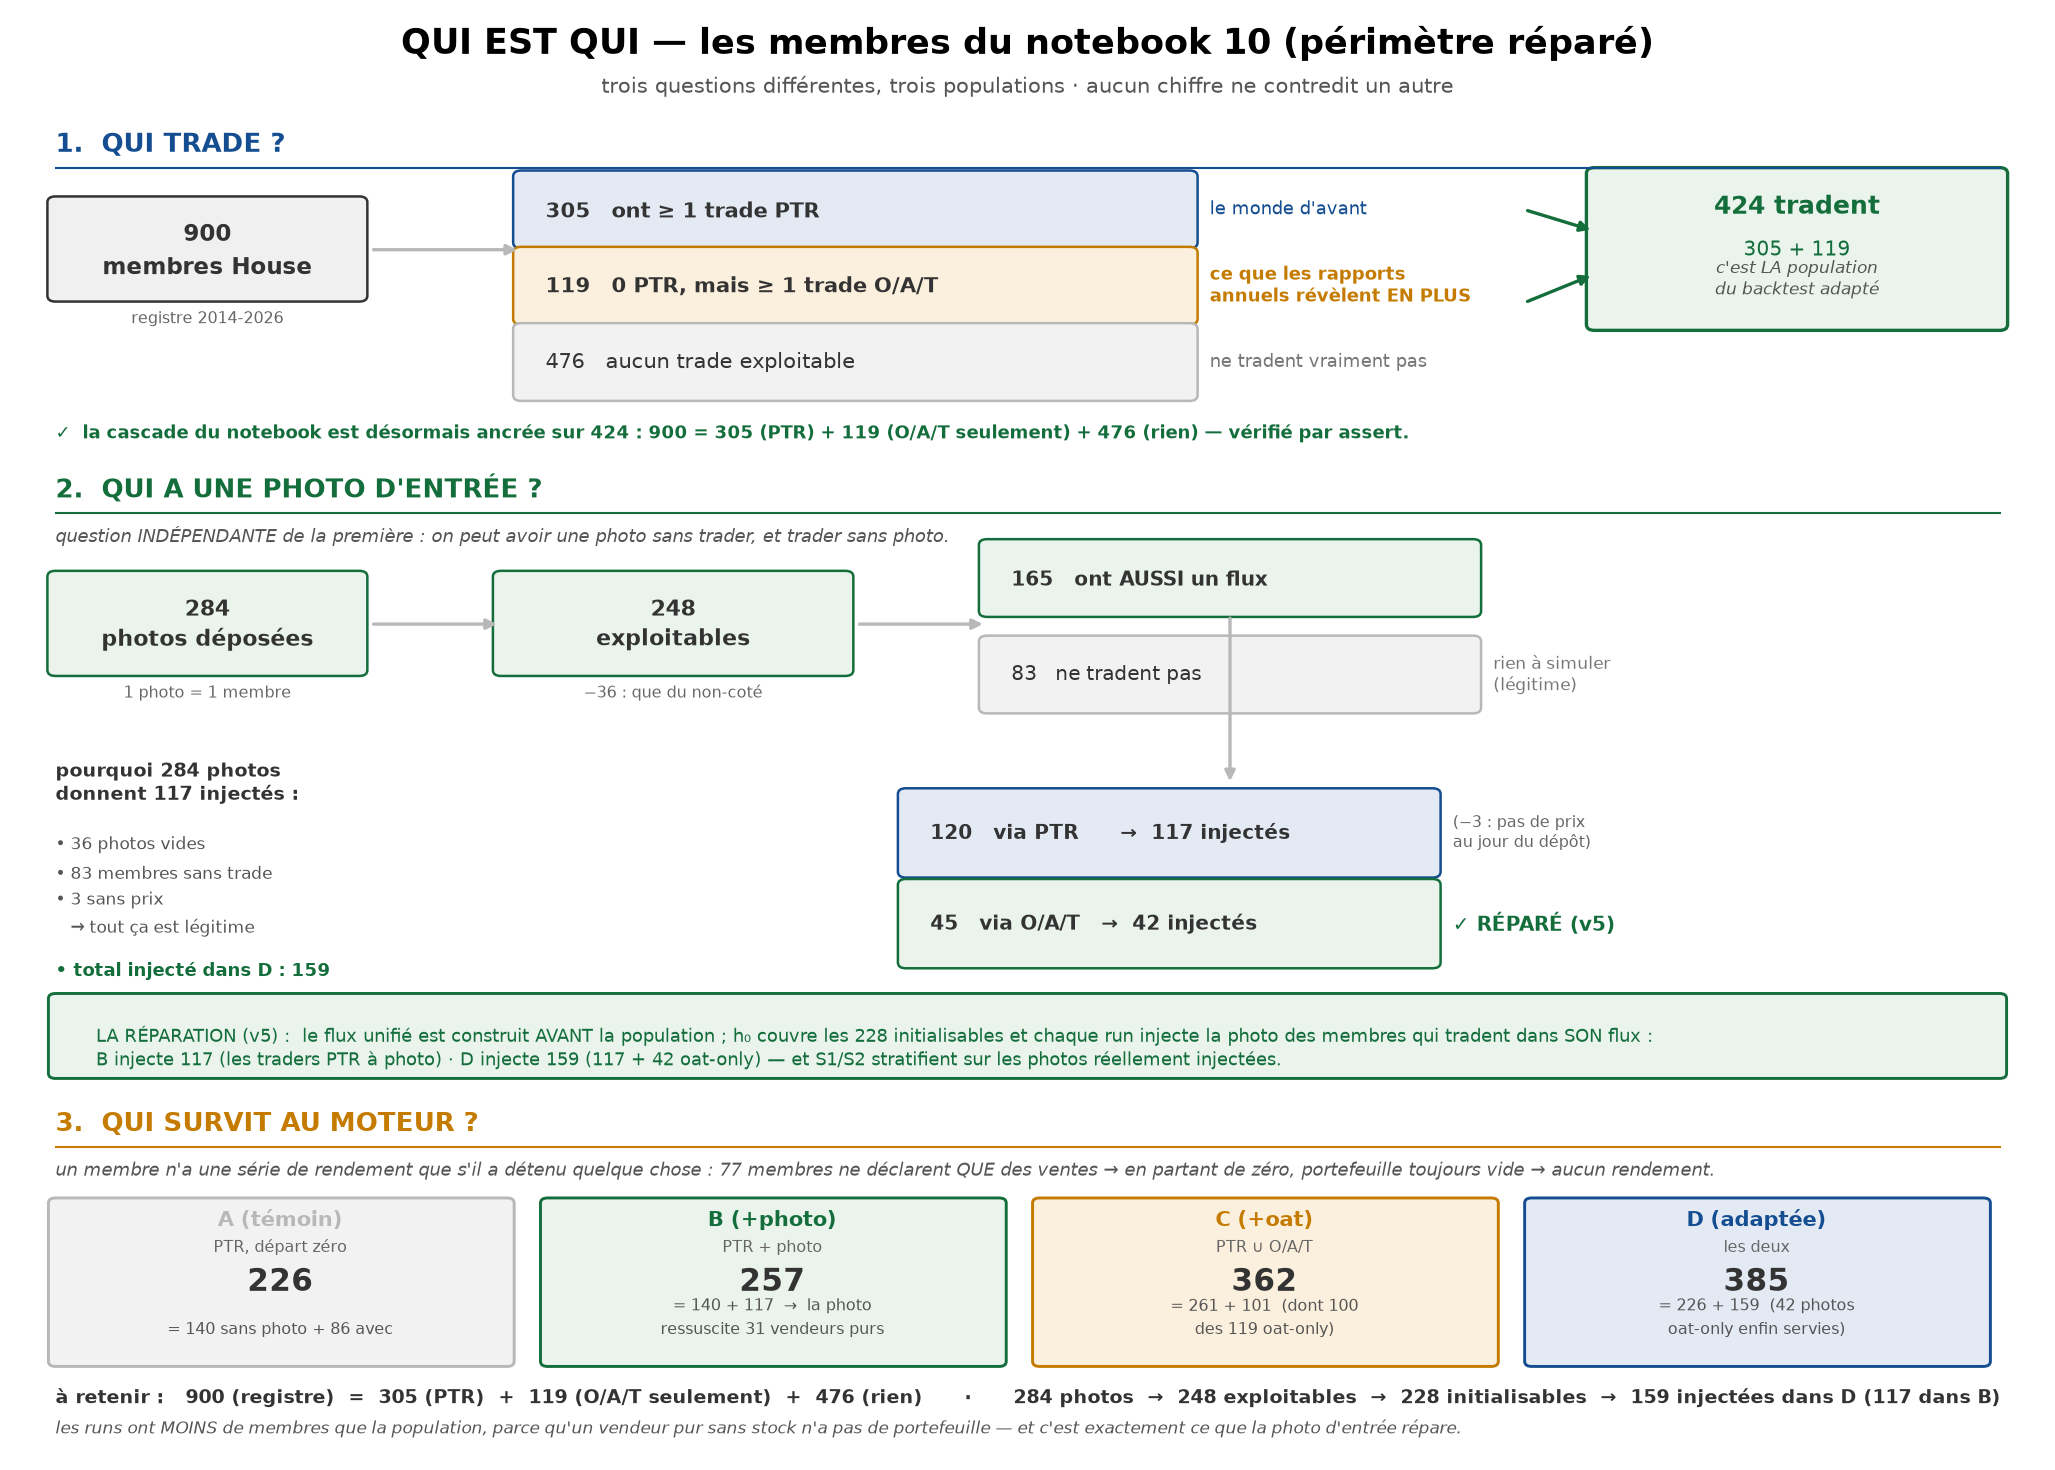
\includegraphics[width=0.9\textwidth]{figures/fig_10_qui_est_qui.png}
\end{center}

\newpage
% ══════════════════════════ PAGE 5 — RÉSULTATS 1/3 ══════════════════════════
\begin{center}
{\Large\bfseries Ce qui en sort (1/3) --- les données, le flux, la population}\\[0.5mm]
{\scriptsize chaque chiffre sort d'une cellule exécutée du notebook (42 cellules, 0 erreur)}
\end{center}

\textbf{\textcolor{bleu}{É1 --- les données}}\quad
table clean : $134\,464$ PTR dont House $122\,814$ $\to$ fenêtre 2013-2026 : $122\,809$ ($315$ membres, $4\,340$ tickers) $\cdot$
photos d'entrée : $284$ déposées $\to$ $248$ membres exploitables ($9\,310$ lignes, $792$ M\$) $\cdot$
O/A/T sans écho PTR : $26\,115$ $\cdot$ map tickers $4\,653$ paires, $0$ conflit $\cdot$ $12$ fourchettes clean$\leftrightarrow$v1, écart $0$ $\cdot$
prix : $3\,927$ tickers chargés ($64$ corrompus exclus) $\to$ \textbf{$107\,976$ trades House avec prix}.

\vspace{2mm}
\noindent\begin{minipage}[t]{0.47\textwidth}\vspace{0pt}
\textbf{\textcolor{orange}{É2 --- le flux de trades, provenance tracée}}
\begin{itemize}
\item[--] entonnoir O/A/T : $26\,115 \to -221$ \og exchange \fg{} $\to -14$ dates hors fenêtre $\to 15\,451$ avec prix $\to -481$ doublons PTR ($490$ appariements) $=$ \textbf{$14\,970$ trades ajoutés} ;
\item[--] flux unifié : \textbf{F $= 122\,946 = 107\,976$ ptr $+ 14\,970$ oat}, \textbf{424 membres} --- $119$ n'existaient QUE dans les rapports annuels ;
\item[--] l'oat pèse le plus en 2023 : $1\,352$ achats oat contre $3\,573$ ptr.
\end{itemize}
\vspace{2mm}
\textbf{\textcolor{bleu}{É3 --- la population (cascade vérifiée par assert)}}
\begin{itemize}
\item[--] $900 = 305$ (vus par les PTR) $+ 119$ (uniquement O/A/T) $+ 476$ (ne tradent pas) \checkmark ;
\item[--] les \textbf{424} traders se partagent en \textbf{165 G\_photo} $/$ \textbf{259 G\_zéro} ($165 + 259 = 424$ \checkmark) ;
\item[--] le schéma complet \og qui est qui \fg{} : page 4.
\end{itemize}
\end{minipage}\hfill
\begin{minipage}[t]{0.50\textwidth}\vspace{0pt}
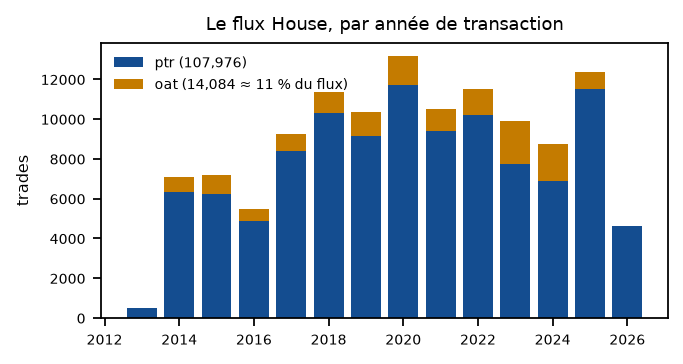
\includegraphics[width=\linewidth]{figures/fig_10_flux.png}\\[1mm]
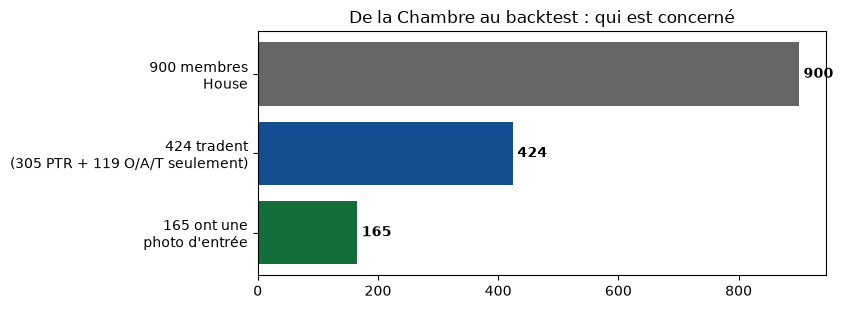
\includegraphics[width=\linewidth]{figures/fig_10_entonnoir.png}
\end{minipage}

\newpage
% ══════════════════════════ PAGE 6 — RÉSULTATS 2/3 ══════════════════════════
\begin{center}
{\Large\bfseries Ce qui en sort (2/3) --- le portefeuille d'entrée, le moteur, les 4 runs}
\end{center}

\noindent\begin{minipage}[t]{0.47\textwidth}\vspace{0pt}
\textbf{\textcolor{vert}{É4 --- le portefeuille d'entrée $h_0$}}
\begin{itemize}
\item[--] \textbf{228 membres initialisables} (sur 248 à photo exploitable), $7\,797$ lignes, \textbf{75,3\,\%} de la valeur convertie en parts ;
\item[--] \textbf{159} tradent ($\in$ 424) $\to$ injectables ; les 69 autres n'ont rien à simuler ;
\item[--] recalculé à la main : ARAIX $32\,500\,\$ \div 59{,}47\,\$ = 546{,}52$ parts \checkmark $\cdot$ AA $8\,000\,\$ \div 30{,}58\,\$ = 261{,}64$ parts \checkmark ;
\item[--] valeur initialisée par membre : médiane \textbf{$387\,505$ \$}, max $78{,}3$ M\$ (G000599).
\end{itemize}
\vspace{2mm}
\textbf{\textcolor{grisf}{É5 --- le moteur et les 4 runs}}
\begin{center}\small
\begin{tabular}{@{}lrrr@{}}
\toprule
run & membres & photos inj. & tronqué \\
\midrule
A (témoin) & 226 & 0 & 937 M\$ \\
B ($+$photo) & 257 & 117 & 897 M\$ \\
C ($+$oat) & 362 & 0 & 1\,179 M\$ \\
\textbf{D (adaptée)} & \textbf{385} & \textbf{159} & 1\,121 M\$ \\
\bottomrule
\end{tabular}
\end{center}
\begin{itemize}
\item[--] \textbf{(i)} fil rouge (G000599) refait en double boucle naïve : $869$ rendements identiques au moteur ;
\item[--] \textbf{(ii)} photo seule $\Rightarrow r = 0$ exactement au jour de l'injection --- un apport n'est jamais une performance ;
\item[--] \textbf{(iii)} B $\equiv$ A pour les membres sans photo injectée (50/140 contrôlés) ;
\item[--] pourquoi 226 $<$ 305 : \textbf{77 vendeurs purs} (aucun achat) n'ont jamais de portefeuille en partant de zéro --- la photo en ressuscite 31 dans B ; D $= 385$ ($+42$ photos oat-only servies).
\end{itemize}
\end{minipage}\hfill
\begin{minipage}[t]{0.50\textwidth}\vspace{0pt}
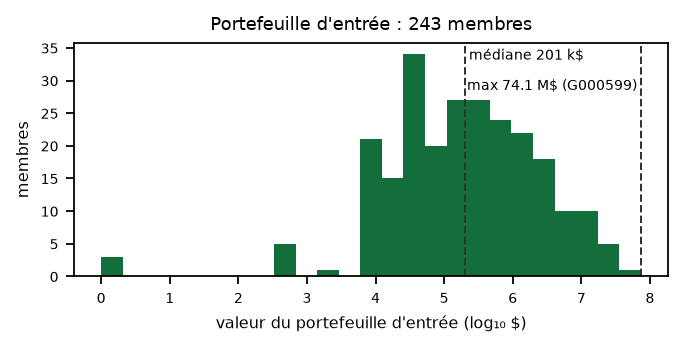
\includegraphics[width=\linewidth]{figures/fig_10_h0_couverture.png}\\[1mm]
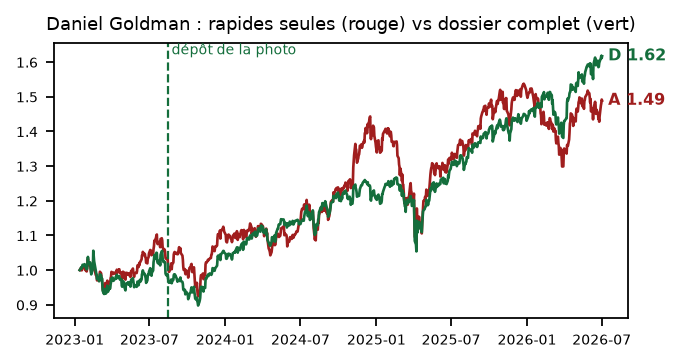
\includegraphics[width=\linewidth]{figures/fig_10_filrouge.png}\\[1mm]
\begin{center}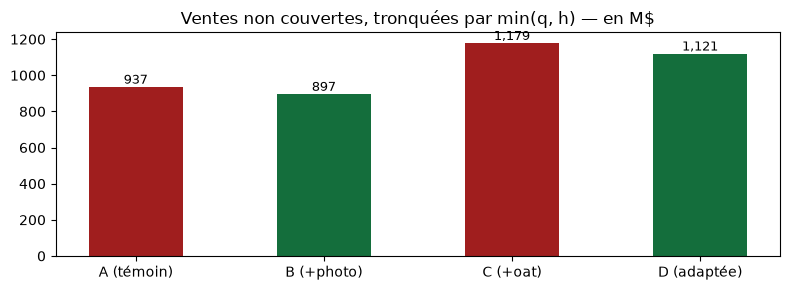
\includegraphics[width=0.8\linewidth]{figures/fig_10_troncature.png}\end{center}
\end{minipage}

\newpage
% ══════════════════════════ PAGE 7 — RÉSULTATS 3/3 ══════════════════════════
\begin{center}
{\Large\bfseries Ce qui en sort (3/3) --- la stratégie, le mélange, le verdict}
\end{center}

\noindent\begin{minipage}[t]{0.49\textwidth}\vspace{0pt}
\textbf{\textcolor{bleu}{É6 --- le tableau central}} {\scriptsize (11 années, seuil $t_{10} \approx 1{,}81$)}
\begin{center}\scriptsize
\begin{tabular}{@{}lrrlrrr@{}}
\toprule
run $\cdot$ poids & excès/an & $t$ & gagn. & $\beta$ & $\alpha$/an & $t_{\text{ap}}$ \\
\midrule
A $\cdot$ 1/K & $+0{,}9$ & $0{,}37$ & 4/11 & $0{,}99$ & $+0{,}6$ & $0{,}28$ \\
A $\cdot$ i-v & $-0{,}3$ & $-0{,}11$ & 4/11 & $1{,}00$ & $-0{,}5$ & $-0{,}27$ \\
\textbf{B $\cdot$ 1/K} & $\mathbf{+6{,}6}$ & $\mathbf{0{,}85}$ & 5/11 & $0{,}98$ & $+5{,}2$ & $\mathbf{1{,}55}$ \\
B $\cdot$ i-v & $+3{,}1$ & $0{,}60$ & 5/11 & $0{,}93$ & $+3{,}3$ & $1{,}33$ \\
C $\cdot$ 1/K & $-0{,}0$ & $-0{,}02$ & 4/11 & $0{,}92$ & $+0{,}9$ & $0{,}54$ \\
C $\cdot$ i-v & $-1{,}4$ & $-0{,}81$ & 5/11 & $0{,}83$ & $+0{,}9$ & $0{,}48$ \\
\textbf{D $\cdot$ 1/K} & $+0{,}7$ & $0{,}31$ & 4/11 & $0{,}89$ & $+1{,}7$ & $\mathbf{0{,}96}$ \\
D $\cdot$ i-v & $-0{,}6$ & $-0{,}31$ & 4/11 & $0{,}82$ & $+1{,}7$ & $0{,}87$ \\
\bottomrule
\end{tabular}
\end{center}
\begin{itemize}
\item[--] \textbf{l'éligibilité du 05b change tout} : l'ancienne règle ($n_{\text{trades}} \ge 10$, run antérieur) donnait un témoin à $-1{,}9\,\%$/an ($t\,{-}1{,}55$) ; celle du 05b : $+0{,}9\,\%$ ($t\,0{,}37$) ;
\item[--] \textbf{inverse-vol perd contre 1/K sur toutes les lignes} ;
\item[--] meilleure ligne : \textbf{B $\cdot$ 1/K, $+6{,}6\,\%$/an} --- $t = 0{,}85$, 5/11 années : non significatif ;
\item[--] éligibles : A $42 \to 184$ $\cdot$ D $50 \to 327$ ; $K^*$ : B verrouille $4$, D se fixe à $6$ depuis 2022 ; oracle bloc 2018 recalculé à la main $\equiv$ moteur \checkmark ; sélection A vs D : change à \textbf{11/11 coupes}.
\end{itemize}
\textbf{\textcolor{orange}{É7 --- S1/S2, le mélange}}
\begin{itemize}
\item[--] \textbf{S1} : le top-$K$ sur-représente G\_photo certaines années --- 2020 : $80\,\%$ vs $30\,\%$ des éligibles $\cdot$ 2021 : $80\,\%$ vs $33\,\%$ $\cdot$ 2022 : $83\,\%$ vs $36\,\%$ --- et $0\,\%$ d'autres (2017, 2019, 2023, 2025) : le mélange pèse réellement ;
\item[--] \textbf{S2} (chaque groupe séparément, 1/K) : A$\cdot$photo $t\,0{,}12$ $\cdot$ A$\cdot$zéro $-0{,}46$ $\cdot$ D$\cdot$photo $-0{,}43$ $\cdot$ D$\cdot$zéro $0{,}60$ ($t_{\text{appr}}$ \textbf{1,59}) --- aucun verdict de strate ne contredit le mixte ;
\item[--] honnêteté : avant la réparation, D$\cdot$zéro affichait $t_{\text{appr}}$ 1,76 --- \textbf{en partie un artefact d'étiquetage} (40 membres à photo étaient classés \og zéro \fg).
\end{itemize}
\textbf{\textcolor{rouge}{É8 --- verdict}}
\begin{itemize}
\item[--] aucune configuration ne franchit le seuil ($\max t = 0{,}85$ ; $\max t_{\text{appr}} = 1{,}59$ en strate) : \textbf{pas d'alpha démontrable}, robuste au poids, à la strate, au mélange --- et au périmètre ;
\item[--] mais l'adaptée reste \textbf{plus propre} ($\beta$ $0{,}99 \to 0{,}89$, $t_{\text{appr}}$ $+0{,}28 \to +0{,}96$) et l'effet photo (B) est la meilleure ligne du tableau ;
\item[--] caveats : O/A/T datés à la transaction (divulgués $\sim$374 j après, notebook V1) $\cdot$ double comptage possible pré-dépôt $\cdot$ non-coté hors périmètre $\cdot$ \texttt{prices\_v2} intact.
\end{itemize}
\end{minipage}\hfill
\begin{minipage}[t]{0.48\textwidth}\vspace{0pt}
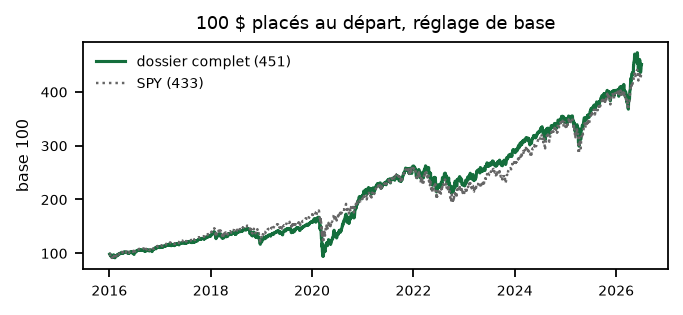
\includegraphics[width=\linewidth]{figures/fig_10_nav.png}\\[1mm]
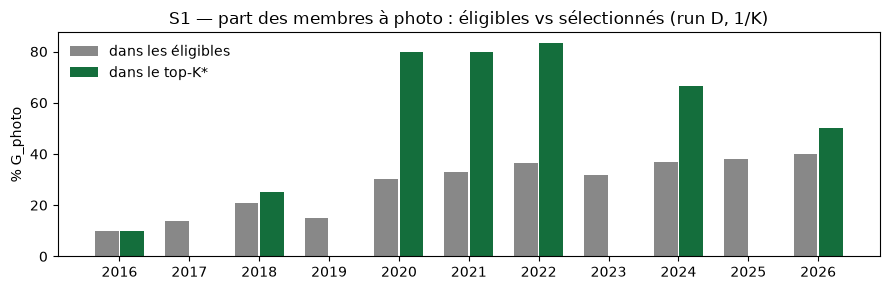
\includegraphics[width=\linewidth]{figures/fig_10_s1.png}\\[1mm]
\begin{center}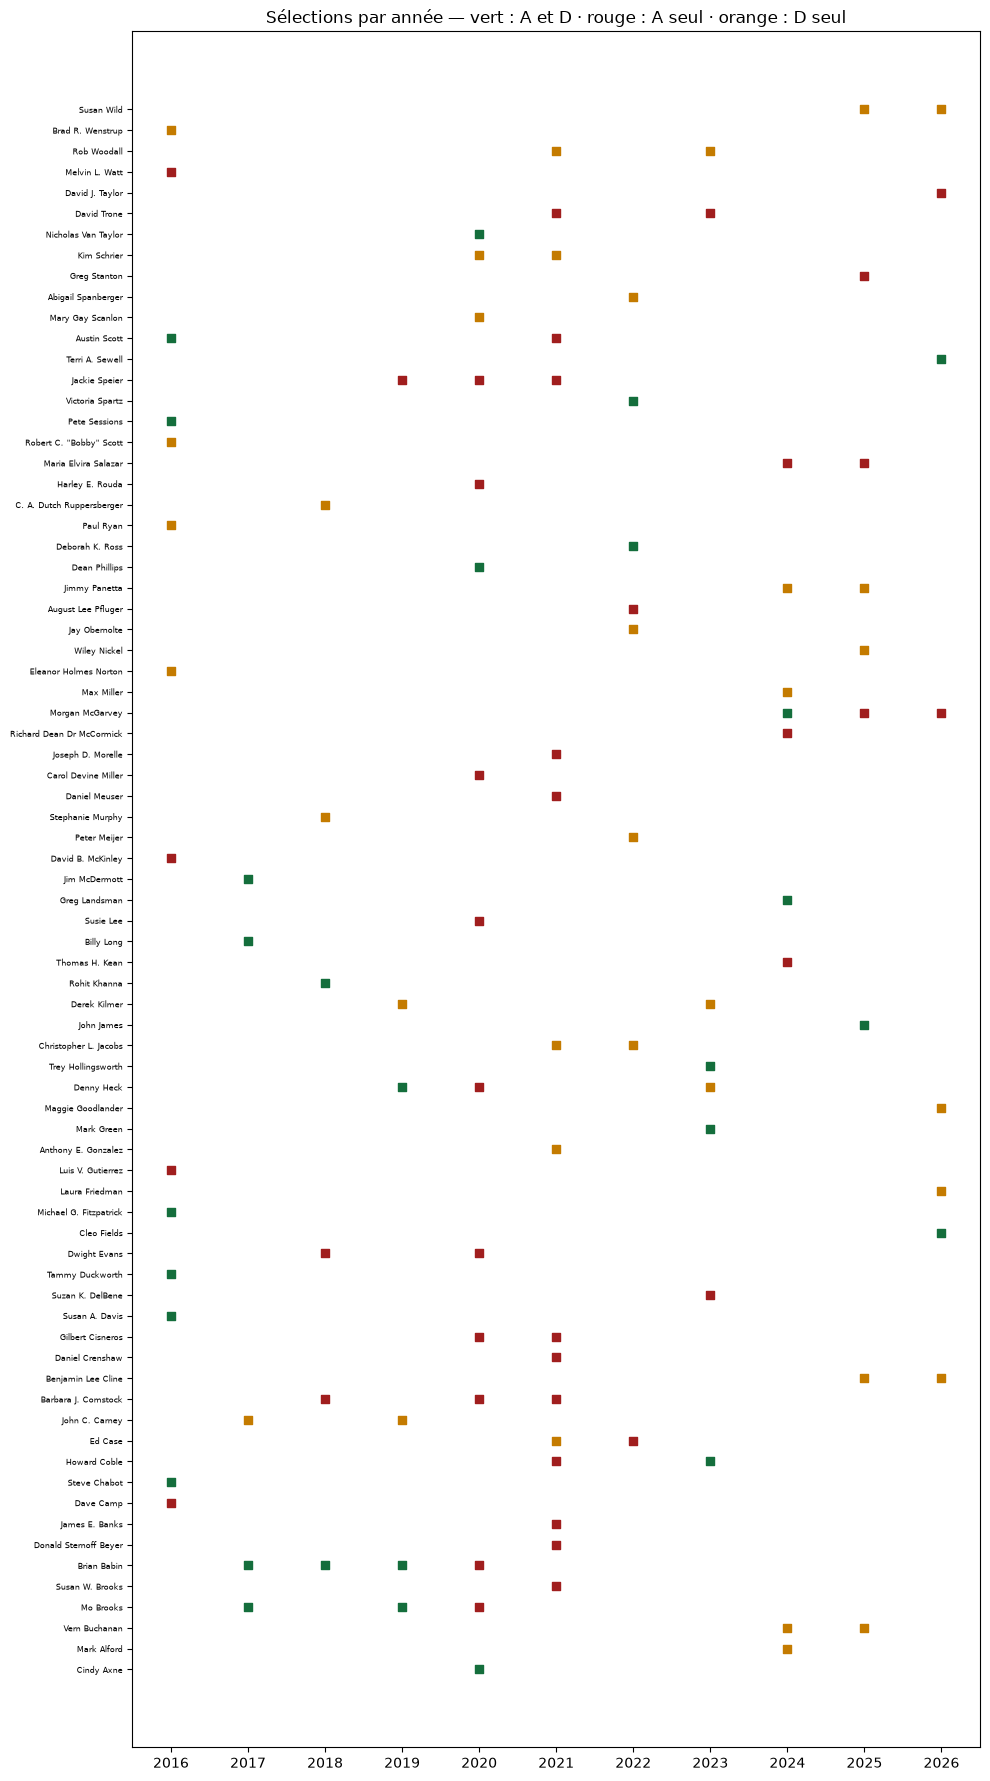
\includegraphics[width=0.85\linewidth,height=6.2cm,keepaspectratio]{figures/fig_10_composition.png}\end{center}
\end{minipage}

\end{document}
